% !Mode:: "TeX:UTF-8"
%!TEX program = xelatex

\documentclass[bwprint]{gmcmthesis}

\hypersetup{hidelinks}

\usepackage{siunitx}
\usepackage{tikz}
\usetikzlibrary{arrows.meta,positioning,shapes.geometric}
\usepackage[noend]{algpseudocode}
\usepackage{algorithmicx,algorithm}
\floatname{algorithm}{算法}
\renewcommand{\algorithmicrequire}{\textbf{输入:}}
\renewcommand{\algorithmicensure}{\textbf{输出:}}

% 第一问现有图位于仓库上一级目录
\graphicspath{{figures/}{../first_answer/figures/}}

% ====================== 参赛信息 ======================
\title{服务于脑机接口与精神性疾病诊断的脑电图计算模型}
\baominghao{\hspace{6em} 待填写}
\schoolname{\hspace{5.8em} 待填写}
\membera{\hspace{6em} 乔逸帆}
\memberb{\hspace{6em} 王佳兴}
\memberc{\hspace{6em} 杨凯}
% =====================================================

\newcommand{\R}{\mathbb{R}}
\newcommand{\EEG}{\mathrm{EEG}}
\newcommand{\ERP}{\mathrm{ERP}}
\newcommand{\Pzero}{\mathrm{P0}}
\newcommand{\Wzero}{\mathrm{W0}}
\newcommand{\TODO}[1]{\textcolor{red!70!black}{\textbf{[TODO: #1]}}}
\newcommand{\PENDING}[1]{\textcolor{gray}{\textbf{[待定稿：#1]}}}

\begin{document}

% 生成封面与标题页
\maketitle

% 摘要
\begin{abstract}
本文针对脑机接口与精神性疾病诊断中的脑电图计算建模问题，围绕脑电信号的保真降噪、视觉诱发响应提取、神经生成机制建模及认知过程建模展开研究。

针对问题一，本文首先对Fz、F3、F4三通道脑电信号进行刺激事件对齐与基线校正，并构建“基础保真滤波--试次质量加权--候选响应子空间平滑”的分层预处理框架。为避免过度降噪破坏弱视觉响应，进一步采用已知波形注入、分块交叉验证、分半稳定性与预处理敏感性分析对候选方法进行约束选择；在此基础上提取不同实验项目、不同刺激条件下的事件相关电位，并采用低阶高斯基函数进行曲线参数化拟合。

针对问题二，\TODO{根据后续LGN--皮层--头皮生成模型补写：核心方程、关键参数、左右三角刺激差异的机制解释与验证结果。}

针对问题三，\TODO{根据后续认知过程模型补写：状态变量、模型结构、参数估计、实验验证与应用意义。}

最终，本文形成从“数据预处理--有效响应提取--神经机制解释--认知状态建模”的统一计算框架，为非侵入式脑机接口及神经精神疾病相关脑电研究提供可解释的建模路径。

\noindent\textbf{关键词：}脑电图；脑机接口；事件相关电位；保真降噪；神经计算模型；视觉认知
\end{abstract}


\pagestyle{plain}

% 按参考模板与上一届优秀论文结构组织正文：
% 一 问题重述 → 二 模型的假设 → 三 问题分析 → 四 符号说明
% → 五 模型的建立与求解 → 六 模型评价 → 七 结论
\section{问题重述}

\subsection{问题背景}

脑电图（Electroencephalography，EEG）能够以非侵入方式记录大量神经元群体活动所形成的头皮电位变化，是连接基础神经科学、脑机接口和神经精神疾病研究的重要观测手段。与单纯依靠统计学习完成“输入—标签”映射不同，本题更关注脑电信号背后的\textbf{生成机制与认知机制}：一方面，需要从含有强伪影的原始EEG中恢复与视觉刺激有关的微弱响应；另一方面，还需要建立从视觉通路、皮层神经群体活动到头皮电极观测的计算联系，并进一步讨论视觉信息与记忆、认知状态之间的动态耦合。

题目给出两个视觉认知实验项目。实验项目I中，受试者在目标出现前已经知道目标位置，主要等待目标出现；实验项目II中，受试者事先不知道目标位于左侧还是右侧，只知道视觉提示的三角形方向。两个项目均在额区F3、Fz、F4记录EEG，因此同一视觉刺激在不同任务条件下的脑电差异，既可能包含直接视觉响应，也可能混合注意、预期、记忆匹配等高层认知因素。

\subsection{实验数据说明}

题目提供四组实验数据：
\[
\texttt{VisualCogA\_Task-1.mat},\quad
\texttt{VisualCogA\_Task-2.mat},\quad
\texttt{VisualCogB\_Task-1.mat},\quad
\texttt{VisualCogB\_Task-2.mat},
\]
采样频率均为$256\,\mathrm{Hz}$。每组数据包含10个记录通道，其中Fz、F3、F4为原始EEG，视觉提示通道用于标记左、右三角提示，目标应答通道记录实际点击行为，另有时间戳等辅助信息。题目同时给出了设备自带滤波后的FzDecon、F3Decon、F4Decon，但明确指出该处理可能在去除干扰的同时破坏视觉响应特征，因此本文不将其作为主要建模输入，而从原始Fz、F3、F4信号出发独立设计预处理流程。

\subsection{问题一：脑电预处理与有效视觉响应提取}

视觉刺激可能在约$250$--$500\,\mathrm{ms}$形成P300相关晚期响应，但原始EEG同时受到眨眼、运动、慢漂移及高频噪声等多种干扰。问题一要求分别针对实验项目I和项目II设计特定降噪方法，在抑制伪影的同时尽量保留视物形状相关特征，随后提取F3、Fz、F4各观测点的有效视觉响应并拟合相应曲线。

因此，问题一的关键并非“滤得越平滑越好”，而是建立可量化的\textbf{降噪—保真折中准则}，并证明最终处理方法没有因为去噪而系统性削弱潜在视觉成分。

\subsection{问题二：LGN—皮层—头皮EEG生成机制}

问题二要求建立从外侧膝状体核（LGN）到皮层、再到头皮EEG观测的计算模型，并利用该模型解释左、右三角形视觉刺激产生不同脑电信号的形成机制，最终构造能够区分左右视觉刺激响应的特征表示。

该问题本质上要求把“刺激图形的空间结构”与“神经群体响应分布”和“头皮电极观测”连接起来。由于三通道EEG不足以唯一反演真实三维神经源，本文将采用受神经生理约束的低维生成模型，在可辨识性与生理解释之间取得平衡。

\subsection{问题三：视觉认知宏观模型}

问题三要求截取与视觉认知相关联的脑电信号，其终点可位于行为应答前约$100\,\mathrm{ms}$，在问题二脑电形成机制的基础上，同时考虑信号可能来源于海马体、LGN等结构，建立视觉认知的宏观模型，并使用题目提供的EEG进行验证。题目特别指出，应答并不一定正确，也可能出现未及时应答，因此不能直接用行为结果替代认知状态本身。

由此，问题三需要在问题二“直接视觉响应”的基础上进一步引入记忆匹配和认知状态，并把视觉提示、内部认知过程与最终行为应答明确分离。

\section{模型假设}

为保证模型可计算性、可验证性，并避免作出超出题目数据支持范围的生理推断，本文作如下基本假设：

\begin{enumerate}[label=\arabic*.]
    \item \textbf{数据有效性假设。} 题目提供的采样顺序、时间戳、视觉提示标记以及F3、Fz、F4原始脑电记录均真实有效，采集系统在同一记录内保持稳定，不考虑人为篡改和大规模硬件故障。
    \item \textbf{相对幅值可比假设。} 在同一实验数据来源内，各试次由同一记录系统获得，因而可在原始记录单位下比较相对幅值、波形形态和时间位置；由于缺少可靠标定信息，本文不擅自将幅值换算为$\mu\mathrm{V}$。
    \item \textbf{刺激前基线假设。} 短时间刺激前区间可近似代表该试次的局部基线，基线校正主要消除直流偏置和缓慢漂移，不改变刺激后的相对动力学结构。
    \item \textbf{事件锁定假设。} 与视觉提示直接相关的神经响应在重复试次中存在一定的事件锁定共同结构，而部分眼动、肌电和随机背景活动与提示事件不同步，因此跨试次统计能够提高视觉诱发成分的可见度。
    \item \textbf{有限空间可辨识假设。} F3、Fz、F4仅提供三个头皮观测，不足以唯一反演LGN、海马或完整皮层的真实三维电流源。因此问题二、三只建立低维等效神经状态与头皮观测之间的映射，不将模型隐状态解释为唯一的解剖定位结果。
    \item \textbf{任务结构共享假设。} 左、右视觉刺激共享大部分基础视觉通路和观测机制，其差异主要通过刺激空间配置、输入编码或部分神经群体状态体现，从而允许在共享动力学框架下比较左右条件。
    \item \textbf{行为与认知非等价假设。} 目标应答可受动作执行、误操作或反应延迟影响，因此行为正确与否不直接等同于认知识别成功与否；问题三中行为通道仅作为外部辅助观测，不作为潜在认知状态的唯一真值标签。
\end{enumerate}

\section{问题分析}

\subsection{问题一分析}

问题一的核心矛盾并非单纯“最大程度去噪”，而是“在抑制伪影的同时尽可能保留未知的视觉任务特征”。若直接采用强平滑、固定模板回归或过度分解，虽然可降低信号方差，却可能同时削弱P300等晚期成分以及左右刺激之间本就微弱的差异。

因此本文将问题一拆分为四个递进环节：

\begin{enumerate}[label=(\arabic*)]
    \item 建立低偏差的基础预处理，获得可比较的保真参考；
    \item 根据试次质量构造稳健权重，降低异常试次对平均响应的影响；
    \item 构造受约束的候选降噪算子，并通过已知信号注入实验检验“去噪--保真”权衡；
    \item 在冻结的主处理方案上提取ERP，分别分析共同视觉响应与左右刺激差分，并进行低维曲线拟合。
\end{enumerate}

\subsection{问题二分析}

问题二要求从“观测差异”进一步过渡到“生成机制”。因此不能仅依赖分类器，而需要显式建立LGN输入、皮层神经群体状态以及头皮电极观测之间的映射。后续模型应同时满足：具有明确状态变量、能够产生与实测EEG可比较的时间序列、能够解释左右视觉刺激在空间配置或输入结构上的差异，并可通过留出数据验证。

\subsection{问题三分析}

\TODO{根据问题三完整题意与后续代码补充。建议强调：从局部视觉响应机制进一步上升到认知/记忆状态的动态建模，并与问题一、二共享观测接口。}

\section{符号说明}

\begin{table}[H]
\centering
\caption{主要符号及含义}
\begin{tabular}{cl}
\toprule
符号 & 含义\\
\midrule
$x_i^{(e)}(t)$ & 第$i$个试次、电极$e$在时刻$t$的脑电观测\\
$f_s$ & 采样频率，本文数据为$256\,\mathrm{Hz}$\\
$\mathcal{T}_0$ & 刺激前基线时间窗\\
$w_i$ & 第$i$个试次的质量权重\\
$N_{\mathrm{eff}}$ & 加权后的有效样本量\\
$U$ & 候选视觉响应子空间的正交基\\
$P=UU^\top$ & 候选响应子空间投影矩阵\\
$S_\lambda$ & 正则化平滑算子\\
$\bar{x}_{c}^{(e)}(t)$ & 条件$c$下电极$e$的平均事件相关响应\\
$f_K(t)$ & 含$K$个高斯成分的参数化响应曲线\\
\bottomrule
\end{tabular}
\end{table}

\TODO{随问题二、三建模过程补充状态变量、耦合参数、观测矩阵等符号。}

\section{模型的建立与求解}

本节依次给出三个问题的模型建立、参数估计、求解过程与结果分析。三问沿用前述“观测层—机制层—认知层”的递进关系，并共享问题一输出的保真EEG、ERP及参数化曲线接口。

\subsection{问题一的模型建立与求解}

\subsubsection{数据组织与事件对齐}

本文以视觉刺激事件为时间零点，将连续脑电划分为刺激锁定试次。每个试次保留Fz、F3、F4三个通道，采样频率为
\[
f_s=256\,\mathrm{Hz}.
\]
根据现有程序，共得到400个刺激锁定试次，两个实验项目各200个。分析片段覆盖约刺激前$0.2\,\mathrm{s}$至刺激后$0.8\,\mathrm{s}$，并利用刺激前样本进行基线校正。

为避免将实验项目与数学建模“问题一/问题二”混淆，后文将题目中的两类实验任务分别记作“实验项目I”和“实验项目II”。

\subsubsection{基础保真预处理模型}

\paragraph{零相位带通滤波与基线校正}

对第$i$个试次的原始信号$x_i(t)$，先进行$0.5$--$30\,\mathrm{Hz}$四阶Butterworth双向滤波，再做刺激前基线校正，得到基础参考信号
\begin{equation}
x_i^{(0)}(t)
=
\mathcal{B}_{0.5-30}[x_i(t)]
-
\frac{1}{|\mathcal T_0|}
\sum_{\tau\in\mathcal T_0}
\mathcal{B}_{0.5-30}[x_i(\tau)],
\label{eq:p0}
\end{equation}
其中$\mathcal{B}_{0.5-30}$表示零相位带通算子，$\mathcal T_0$为刺激前基线区间。本文将式\eqref{eq:p0}记为基础处理$\Pzero$。

该步骤用于抑制低频漂移及较高频噪声，同时避免相位延迟。由于题目数据未给出可靠的物理单位换算关系，本文后续幅值统一采用“记录单位”。

\paragraph{试次质量加权}

为降低眨眼、运动及突发高幅值波动对平均ERP的影响，本文不直接删除试次，而是根据峰峰值、均方根、一阶差分MAD及异常幅值比例构造质量权重$w_i$。对条件$c$，加权ERP为
\begin{equation}
\bar{x}_c(t)
=
\frac{\sum_{i\in c} w_i x_i^{(0)}(t)}
{\sum_{i\in c} w_i}.
\label{eq:weighted_erp}
\end{equation}

同时定义有效样本量
\begin{equation}
N_{\mathrm{eff}}
=
\frac{\left(\sum_i w_i\right)^2}
{\sum_i w_i^2},
\label{eq:neff}
\end{equation}
用于判断加权结果是否过度依赖少量高权重试次。该质量加权方案记为$\Wzero$。

\subsubsection{候选响应子空间与受约束平滑}

将训练数据中稳定出现的共同响应和左右半差分响应堆叠后进行低维正交分解，取前$r$个方向组成矩阵$U$，并定义投影矩阵
\begin{equation}
P=UU^\top.
\end{equation}

为了尽量保留候选视觉响应子空间，而只对其正交补空间进行平滑，构造
\begin{equation}
\mathcal{D}_{r,\lambda}x
=
Px+(I-P)\widetilde S_\lambda x,
\label{eq:subspace_denoise}
\end{equation}
其中
\begin{equation}
S_\lambda=(I+\lambda D_2^\top D_2)^{-1},
\end{equation}
$D_2$为二阶差分算子，$\lambda$控制平滑强度。

本文在训练折内考察
\[
r\in\{0,2,4\},\qquad
\lambda\in\{1,10,100\},
\]
并与$\Pzero$、$\Wzero$共同构成有限候选集。模型选择只使用训练折信息，以验证折ERP预测误差为准，避免在完整数据上观察曲线后再挑选最有利方法。

\subsubsection{保真约束与模型选择}

仅以输出“更平滑”作为降噪成功标准是不充分的。为检验算法是否同时损伤真实视觉响应，本文在原始片段入口注入已知波形，并将处理后的恢复结果与滤波前真值比较。

定义峰值幅度相对误差
\begin{equation}
E_A=\frac{|\hat A-A|}{|A|},
\end{equation}
以及峰时偏移
\begin{equation}
E_t=|\hat t_p-t_p|.
\end{equation}

预设工程保真门槛为
\[
E_A\le 10\%,\qquad E_t\le 2\ \text{samples}.
\]

现有结果表明：对于宽共同响应，$\Pzero$和两个项目选出的学习型候选幅值误差均约为$8\%$；但对窄反对称响应，$\Pzero$幅值误差约为$2.08\%$，而两个学习型候选均约为$10.8\%$，超过预设保真阈值。因此，尽管学习型候选在部分稳定性指标上有所改善，本文仍选取$\Pzero$作为后续主分析信号，并将$\Wzero$用于稳健ERP辅助估计。

\begin{table}[H]
\centering
\caption{主要候选方法的已知信号保真结果}
\label{tab:q1_fidelity}
\begin{tabular}{lccc}
\toprule
方法 & 宽共同峰幅值误差 & 窄反对称峰幅值误差 & 最大峰时偏移\\
\midrule
$\Pzero$ & 8.09\% & 2.08\% & 0\\
项目I学习型候选 & 8.26\% & 10.80\% & 0\\
项目II学习型候选 & 8.27\% & 10.81\% & 0\\
\bottomrule
\end{tabular}
\end{table}

\subsubsection{视觉诱发响应提取与稳定性检验}

对每个实验项目、刺激条件和电极分别计算ERP，并进一步构造共同响应
\begin{equation}
m(t)=\frac{\bar{x}_{L}(t)+\bar{x}_{R}(t)}{2},
\end{equation}
以及左右差分响应
\begin{equation}
d(t)=\bar{x}_{L}(t)-\bar{x}_{R}(t).
\end{equation}

为避免事后挑选时间窗，主检验固定在$250$--$500\,\mathrm{ms}$晚期窗口。统计上采用记录内分块、双侧符号翻转检验及Holm多重比较校正，并通过移动块重采样给出条件性置信区间。

现有结果显示，质量加权显著提高了共同ERP的分半一致性：实验项目I的平均分半相关系数由$\Pzero$的约$0.554$提高至$\Wzero$的约$0.785$，实验项目II由约$0.920$提高至约$0.985$；但左右差分响应的分半相关仍较低。因此，第一问能够较稳定地支持“共同视觉响应”的存在，而尚不能仅凭传统ERP平均证明稳定的左右形状差异。

在固定晚期窗口中，实验项目II的Fz通道观察到较明显的共同诱发变化，但该效应对滤波及边界上下文存在敏感性。故本文将其表述为“晚期视觉诱发响应”，不直接认定为稳定正向P300。

\subsubsection{响应曲线参数化拟合}

为满足题目“拟合相应曲线”的要求，采用低阶高斯基函数描述ERP：
\begin{equation}
f_K(t)
=
b+\sum_{j=1}^{K}
a_j
\exp\left[
-\frac{(t-\mu_j)^2}{2\sigma_j^2}
\right],
\qquad K\in\{0,1,2\}.
\label{eq:gaussian_fit}
\end{equation}

其中$K=0$表示无明显峰型，$K=1$表示单峰响应，$K=2$表示早期与晚期双成分。模型阶数在开发数据内部选择，并通过分块重采样估计参数区间。

现有12条“实验项目--刺激条件--电极”曲线中，4条选择常数模型、2条选择单高斯模型、6条选择双高斯模型。由于部分曲线参数达到约束边界，本文将高斯参数仅作为观测曲线的低维描述，不直接等价解释为确定的神经生理成分。

% 若需要临时插入当前6页结果PDF的第一页，可取消下面注释：
% \begin{figure}[H]
% \centering
% 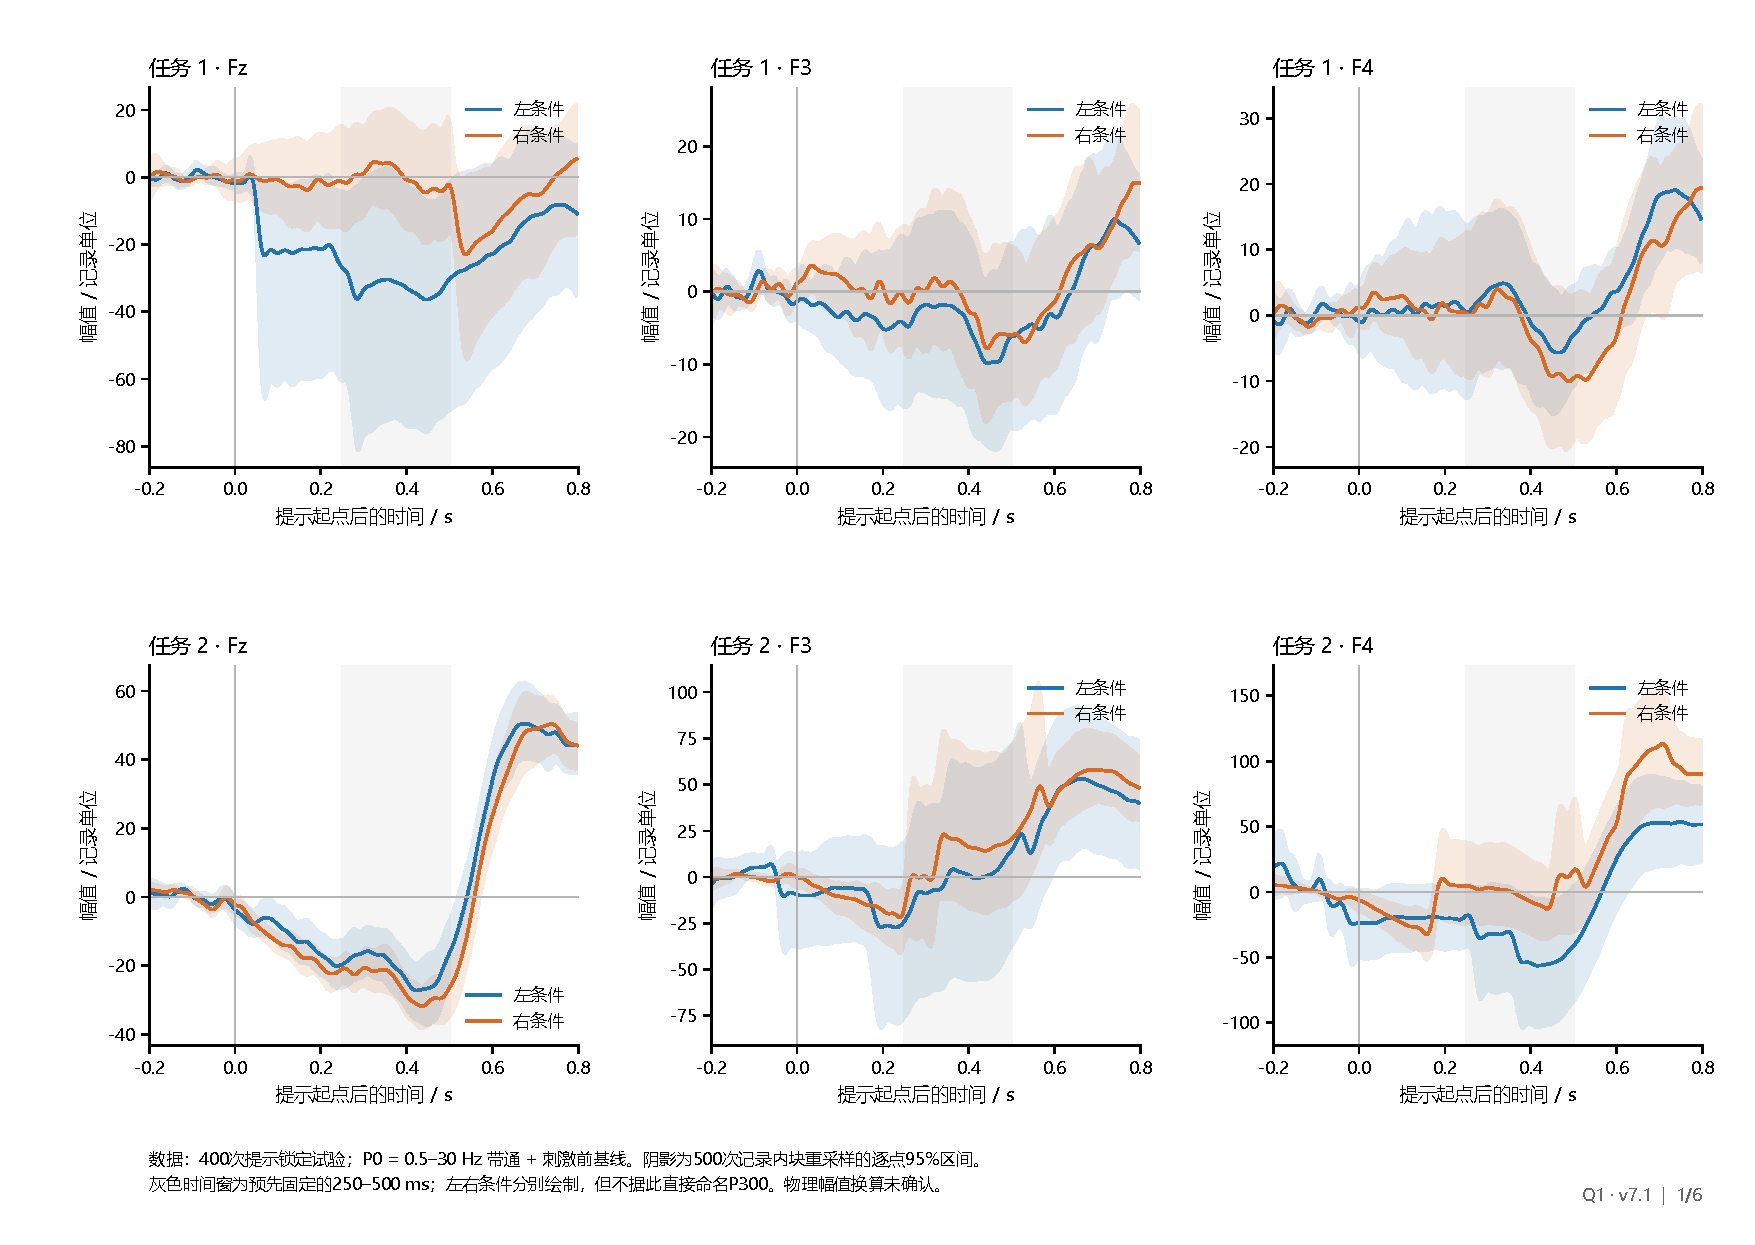
\includegraphics[page=1,width=0.95\textwidth]{q1_results.pdf}
% \caption{问题一主要结果示意}
% \label{fig:q1_results_preview}
% \end{figure}

\subsubsection{问题一小结}

综上，本文建立了以“特征保真”为优先约束的脑电预处理框架。基础零相位带通滤波负责信号级保真，试次质量加权负责提高跨试次稳健性，候选子空间方法则通过训练折评价与人工注入实验接受约束选择。结果表明，复杂平滑方法并未在所有保真指标上优于基础模型，因此本文主动保留$\Pzero$作为后续问题的统一可比输入。

问题一提取出的共同ERP、左右差分ERP以及参数化响应曲线，将作为问题二建立LGN--皮层--头皮生成模型的观测接口。

\section{问题二：LGN--皮层--头皮脑电生成模型}

\subsection{建模目标}

问题二需要从“数据相关性”上升到“生成机制”：建立外界视觉刺激经LGN输入、皮层神经群体动力学到头皮F3/Fz/F4观测的低维计算模型，并解释左、右三角刺激产生不同脑电响应的机制。

\subsection{模型结构}

\TODO{补写模型结构图：视觉刺激编码 $\rightarrow$ LGN输入 $\rightarrow$ 皮层兴奋/抑制神经群体 $\rightarrow$ 头皮观测矩阵。}

建议采用统一状态空间形式：
\begin{align}
\dot{\bm z}(t) &= F\!\left(\bm z(t),\bm u(t);\bm\theta\right),\\
\bm y(t) &= H\bm z(t)+\bm\varepsilon(t),
\end{align}
其中$\bm z(t)$为皮层等效神经状态，$\bm u(t)$为视觉/LGN输入，$H$为从隐状态到F3/Fz/F4的观测矩阵。

\subsection{左右视觉刺激的差异编码}

\TODO{根据第二问实际程序确定：左右三角差异究竟由输入方向、相对位置配置、耦合权重还是空间观测映射表示。正文必须与代码一致，不先写结论。}

\subsection{参数估计与模型求解}

\TODO{补充损失函数、参数约束、训练/验证划分、数值积分方法及初始化。}

\subsection{模型验证}

建议至少包含：
\begin{enumerate}[label=(\arabic*)]
    \item 对留出ERP曲线的时域重建误差；
    \item 三电极空间模式的一致性；
    \item 左右刺激差分的预测能力；
    \item 参数扰动/敏感性分析；
    \item 与简化基线模型的对比。
\end{enumerate}

\subsection{问题二小结}

\TODO{在第二问完成后，用“模型解释了什么、验证到了什么、不能声称什么”三句话收束。}

\section{问题三：视觉认知过程的脑电计算模型}

\subsection{建模目标}

\TODO{先按题目原文补全问题三任务要求，再确定状态变量。不要在题意尚未核实前写疾病诊断性能或行为正确率。}

\subsection{状态变量与认知过程分解}

可预留以下统一框架：
\begin{equation}
\bm s_{t+1}
=
G(\bm s_t,\bm r_t;\bm\phi)
+
\bm\eta_t,
\end{equation}
其中$\bm r_t$为问题二得到的视觉响应表征，$\bm s_t$表示认知/记忆相关低维状态。

\TODO{后续根据最终模型定义视觉输入状态、记忆状态、认知判别状态等具体变量。}

\subsection{参数估计与模型比较}

\TODO{给出完整目标函数、正则项、嵌套验证或留出验证协议。}

\subsection{结果与解释}

\TODO{补写第三问结果。若原始数据没有行为标签、患者标签或临床诊断信息，不得把模型输出写成已验证的临床诊断准确率。}

\subsection{问题三小结}

\TODO{形成从问题一观测层、问题二机制层到问题三认知层的统一闭环。}


\section{模型评价与敏感性分析}

\subsection{模型优点}

\begin{enumerate}[label=(\arabic*)]
    \item \textbf{强调保真而非单纯降噪。} 第一问通过人工已知信号注入显式检查视觉响应幅值和峰时是否被算法破坏。
    \item \textbf{避免信息泄漏。} 学习型预处理和超参数选择在训练折内完成，并将历史测试结果与开发阶段结果区分。
    \item \textbf{统计结论较克制。} 对共同响应、左右差分、P300样晚期成分分别陈述，不以单一显著性结果代替机制结论。
    \item \textbf{便于向后续问题传递。} 第一问输出统一的试次级EEG、ERP和拟合曲线，可直接作为问题二、三的观测接口。
\end{enumerate}

\subsection{模型局限}

\begin{enumerate}[label=(\arabic*)]
    \item 仅有F3、Fz、F4三个通道，不能完成唯一的三维神经源定位；
    \item 当前幅值缺少可靠物理单位换算，因此只在记录单位下解释；
    \item 左右刺激差分的分半稳定性较弱，需要在问题二利用联合时空动力学而非单点均值进一步建模；
    \item 部分晚期响应对滤波边界和慢漂移处理敏感，因此P300生理解释应保持谨慎。
\end{enumerate}

\subsection{敏感性分析}

\TODO{整合问题一已有的滤波、填充、块长度敏感性；问题二、三完成后补充关键参数扰动与模型结构消融。}

\section{结论}

本文围绕视觉刺激条件下的脑电信号分析与计算建模，构建从数据预处理到神经机制解释的分层模型框架。

针对问题一，建立了保真约束的脑电预处理与ERP提取方法。结果表明，质量加权能够提升共同ERP的稳定性，而更复杂的学习型平滑并未在所有人工信号保真测试中通过验收，因此最终采用基础保真处理作为后续统一输入。这一结果说明，在弱脑电特征分析中，模型复杂度并非越高越好，视觉任务相关信息的保留应优先于单纯的平滑程度。

\TODO{问题二完成后补写LGN--皮层--头皮生成机制的主要结论。}

\TODO{问题三完成后补写认知模型的主要结论与脑机接口/精神性疾病研究意义。}

% 参考文献采用模板自带 gmcm.bst
% 当前框架阶段先列出已使用的基础文献，后续在正文中补齐对应 \cite{}。
\nocite{Pernet2020,Luck2017,Bigdely2015,Glomb2022,Steeghs2025,Daume2024,Acebron2005,Azzopardi2014}
\bibliographystyle{gmcm}
\bibliography{reference}

\clearpage
\begin{appendices}

\section{程序与结果文件索引}

\subsection{问题一主要程序}

\begin{itemize}
    \item \texttt{../first\_answer/code/q1\_v7\_core.py}
    \item \texttt{../first\_answer/code/q1\_v7\_pipeline.py}
    \item \texttt{../first\_answer/code/q1\_v7\_statistics.py}
    \item \texttt{../first\_answer/code/q1\_v7\_fitting.py}
    \item \texttt{../first\_answer/code/q1\_v7\_injection.py}
\end{itemize}

\subsection{问题一主要结果文件}

完整数值结果保存在\texttt{../first\_answer/results/}，包括ERP曲线、保真注入结果、分半稳定性、统计检验、敏感性分析及高斯拟合参数。

\subsection{后续程序索引}

\PENDING{第二问、第三问完成后补充对应代码文件、运行命令与关键输出文件。}

\end{appendices}


\end{document}
